\chapter{Kế hoạch quản lý chi tiết}
\section{Kế hoạch quản lý phạm vi}
\subsection{Phạm vi công việc}
\subsubsection{Phạm vi công việc Khảo sát}
\begin{itemize}
    \item \textbf{Tên Công Việc:} Khảo sát
    \item \textbf{Mô tả công việc:}
          \begin{itemize}
              \item Trao đổi những vấn đề mà doanh nghiệp đang gặp phải trong quá trình quản lý Nhân sự - Tiền lương.
              \item Khảo sát về mong muốn, yêu cầu của doanh nghiệp đối với hệ thống.
              \item Tìm hiểu quy trình quản lý Nhân sự - Tiền lương của doanh nghiệp.
          \end{itemize}
    \item \textbf{Các Sản phẩm của công việc:}
          \begin{itemize}
              \item Báo cáo khảo sát chi tiết
              \item Tài liệu mô tả yêu cầu chức năng và phi chức năng
              \item Tài liệu mô tả quy trình nghiệp vụ
              \item Hồ sơ khảo sát hoàn chỉnh
          \end{itemize}
    \item \textbf{Yêu cầu đánh giá:}
          \begin{itemize}
              \item Báo cáo tài liệu phân tích yêu cầu khách hàng phải rõ ràng và dễ hiểu.
              \item Hoàn thành công việc trong thời gian quy định, không quá 5 ngày.
          \end{itemize}
\end{itemize}
\subsubsection{Phạm vi công việc Khảo sát}
\begin{itemize}
    \item \textbf{Tên Công Việc:} Khảo sát
    \item \textbf{Mô tả công việc:}
          \begin{itemize}
              \item Trao đổi những vấn đề mà doanh nghiệp đang gặp phải trong quá trình quản lý Nhân sự - Tiền lương.
              \item Khảo sát về mong muốn, yêu cầu của doanh nghiệp đối với hệ thống.
              \item Tìm hiểu quy trình quản lý Nhân sự - Tiền lương của doanh nghiệp.
          \end{itemize}
    \item \textbf{Các Sản phẩm của công việc:}
          \begin{itemize}
              \item Báo cáo khảo sát chi tiết
              \item Tài liệu mô tả yêu cầu chức năng và phi chức năng
              \item Tài liệu mô tả quy trình nghiệp vụ
              \item Hồ sơ khảo sát hoàn chỉnh
          \end{itemize}
    \item \textbf{Yêu cầu đánh giá:}
          \begin{itemize}
              \item Báo cáo tài liệu phân tích yêu cầu khách hàng phải rõ ràng và dễ hiểu.
              \item Hoàn thành công việc trong thời gian quy định, không quá 5 ngày.
          \end{itemize}
\end{itemize}

\subsubsection{Phạm vi công việc Phân tích và thiết kế hệ thống}
\begin{itemize}
    \item \textbf{Tên Công Việc:} Phân tích và thiết kế hệ thống
    \item \textbf{Mô tả công việc:}
          \begin{itemize}
              \item Phân tích từ yêu cầu và vấn đề khách hàng thành các yêu cầu cho hệ thống
              \item Thiết kế hệ thống dựa trên kết quả phân tích
          \end{itemize}
    \item \textbf{Các sản phẩm của công việc:}
          \begin{itemize}
              \item Báo cáo phân tích quy trình nghiệp vụ chi tiết cho các phần:
                    \begin{itemize}
                        \item Quản lý nhân sự
                        \item Quản lý phần chấm công
                        \item Quản lý hồ sơ tiền lương
                        \item Thanh toán lương
                    \end{itemize}
              \item Báo cáo phân tích yêu cầu chi tiết cho các phần:
                    \begin{itemize}
                        \item Yêu cầu giao diện
                        \item Yêu cầu chức năng
                    \end{itemize}
              \item Các biểu đồ thiết kế hệ thống bao gồm:
                    \begin{itemize}
                        \item Biểu đồ usecase
                        \item Biểu đồ lớp
                        \item Biểu đồ tuần tự
                        \item Biểu đồ hoạt động
                    \end{itemize}
              \item Thiết kế cơ sở dữ liệu chi tiết cho các phần:
                    \begin{itemize}
                        \item Nhân sự
                        \item Hồ sơ lương
                        \item Phần chấm công
                        \item Thanh toán lương
                    \end{itemize}
              \item Các thiết kế giao diện chi tiết cho các phần:
                    \begin{itemize}
                        \item Quản lý nhân sự
                        \item Quản lý hồ sơ lương
                        \item Quản lý phần chấm công
                        \item Thanh toán lương
                    \end{itemize}
              \item Báo cáo tổng hợp và lập bản báo cáo yêu cầu hệ thống
              \item Báo cáo tổng hợp và lập bản báo cáo kiến trúc hệ thống
              \item Báo cáo tổng hợp và lập bản thiết kế giao diện
              \item Hồ sơ phân tích thiết kế
          \end{itemize}
    \item \textbf{Yêu cầu đánh giá:}
    \begin{itemize}
        \item Tài liệu phân tích và thiết kế phải đúng theo tài liệu phân tích yêu cầu khách hàng
        \item Hoàn thành công việc trong thời gian quy định, không quá 15 ngày
    \end{itemize}
\end{itemize}
\subsubsection{Phạm vi công việc Xây dựng và phát triển}
\begin{itemize}
    \item \textbf{Tên Công Việc:} Xây dựng và phát triển
    \item \textbf{Mô tả công việc:}
    \begin{itemize}
        \item Lập trình các chức năng của hệ thống
        \item Tạo tài liệu thiết kế hệ thống
    \end{itemize}
    \item \textbf{Các sản phẩm của công việc:}
    \begin{itemize}
        \item Hệ thống hoàn chỉnh bao gồm các phần:
        \begin{itemize}
            \item Cơ sở dữ liệu
            \item Front-end
            \item Back-end
        \end{itemize}
        \item Báo cáo chi tiết về quá trình xây dựng và phát triển hệ thống
        \item Tài liệu hướng dẫn sử dụng và quản lý hệ thống
    \end{itemize}
    \item \textbf{Yêu cầu đánh giá:}
    \begin{itemize}
        \item Hoàn thành lập trình ứng dụng đúng với tài liệu đặc tả và thiết kế hệ thống
        \item Hoàn thành công việc trong thời gian quy định, không quá 25 ngày
    \end{itemize}
\end{itemize}

\subsubsection{Phạm vi công việc Kiểm thử}
\begin{itemize}
    \item \textbf{Tên Công Việc:} Kiểm thử
    \item \textbf{Mô tả công việc:}
    \begin{itemize}
        \item Kiểm tra và thử nghiệm hệ thống để đảm bảo tính chính xác và đáng tin cậy của hệ thống
        \item Xác định và khắc phục lỗi hoặc sai sót trong chức năng và giao diện hệ thống so với tài liệu đặc tả và yêu cầu ban đầu
    \end{itemize}
    \item \textbf{Các sản phẩm của công việc:}
    \begin{itemize}
        \item Phần mềm hoàn chỉnh sau kiểm thử bao gồm:
        \begin{itemize}
            \item Hồ sơ kiểm thử hoàn chỉnh
            \item Testcase chi tiết cho các chức năng của hệ thống
            \item Kết quả chạy testcase
            \item Báo cáo kiểm tra và sửa lỗi
            \item Báo cáo chi tiết về quá trình kiểm thử và sửa lỗi
            \item Tài liệu hướng dẫn sử dụng và quản lý phần mềm sau kiểm thử
        \end{itemize}
    \end{itemize}
    \item \textbf{Yêu cầu đánh giá:}
    \begin{itemize}
        \item Hoàn thành việc kiểm thử hệ thống, đảm bảo không còn bất kỳ sai sót nào
        \item Hoàn thành công việc trong thời gian quy định, không quá 7 ngày
    \end{itemize}
\end{itemize}
\subsubsection{Phạm vi công việc Triển khai và Bàn giao}
\begin{itemize}
    \item \textbf{Tên Công Việc:} Triển khai và bàn giao
    \item \textbf{Mô tả công việc:}
    \begin{itemize}
        \item Tiến hành cài đặt hệ thống
        \item Hướng dẫn sử dụng hệ thống
        \item Bàn giao hệ thống cho khách hàng
    \end{itemize}
    \item \textbf{Các sản phẩm của công việc:}
    \begin{itemize}
        \item Phần mềm hoàn chỉnh sau chuyển giao bao gồm:
        \begin{itemize}
            \item Hồ sơ triển khai và chuyển giao hoàn chỉnh
            \item Tài liệu hướng dẫn sử dụng
            \item Báo cáo chi tiết về quá trình bàn giao và cài đặt
            \item Báo cáo chi tiết về quá trình đào tạo và sử dụng
        \end{itemize}
        \item Báo cáo chi tiết về quá trình chuyển giao
        \item Tài liệu hướng dẫn sử dụng và quản lý hệ thống sau khi chuyển giao
    \end{itemize}
    \item \textbf{Yêu cầu đánh giá:}
    \begin{itemize}
        \item Hoàn thành việc cài đặt hệ thống và hướng dẫn sử dụng thành công
        \item Bàn giao hệ thống đúng với yêu cầu của khách hàng
        \item Hoàn thành công việc trong thời gian quy định, không quá 8 ngày
    \end{itemize}
\end{itemize}
\subsection{Sơ đồ phân rã công việc}
\begin{figure}[H]
    \centering
    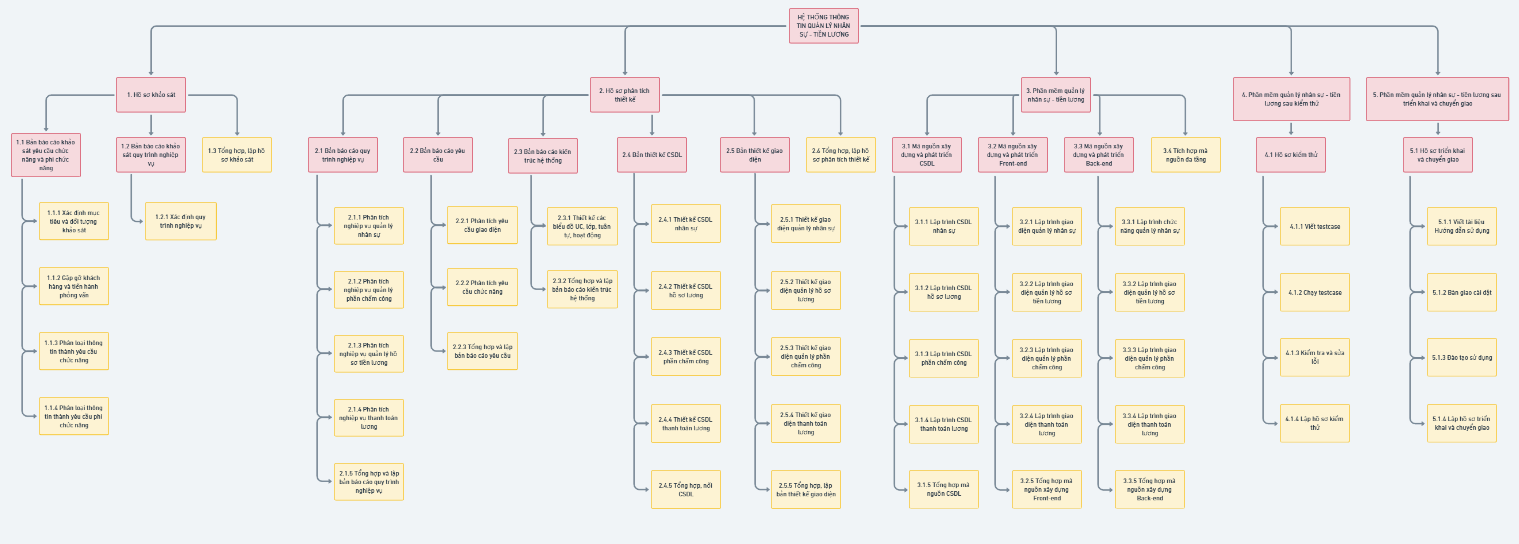
\includegraphics[width=\textwidth]{images/sodophanratongquat.png}
    \caption{Sơ đồ phân rã công việc}
\end{figure}
\begin{figure}[H]
    \centering
    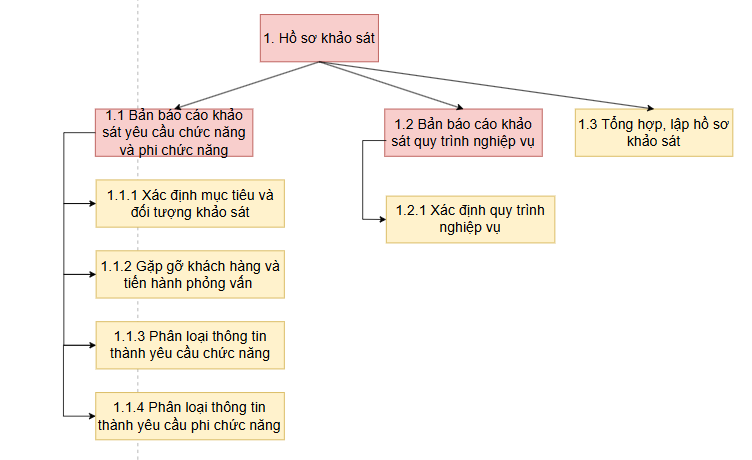
\includegraphics[width=\textwidth]{images/hskhaosat.png}
    \caption{Phân rã chi tiết Hồ sơ khảo sát}
\end{figure}
\begin{figure}[H]
    \centering
    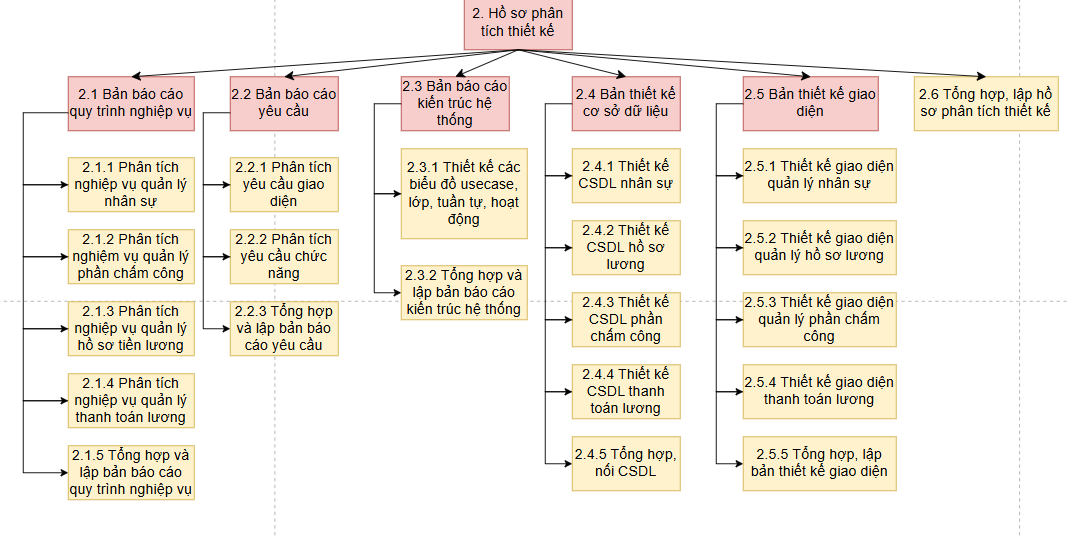
\includegraphics[width=\textwidth]{images/hspttk.png}
    \caption{Phân rã chi tiết hồ sơ phân tích thiết kế}
\end{figure}
\begin{figure}[H]
    \centering
    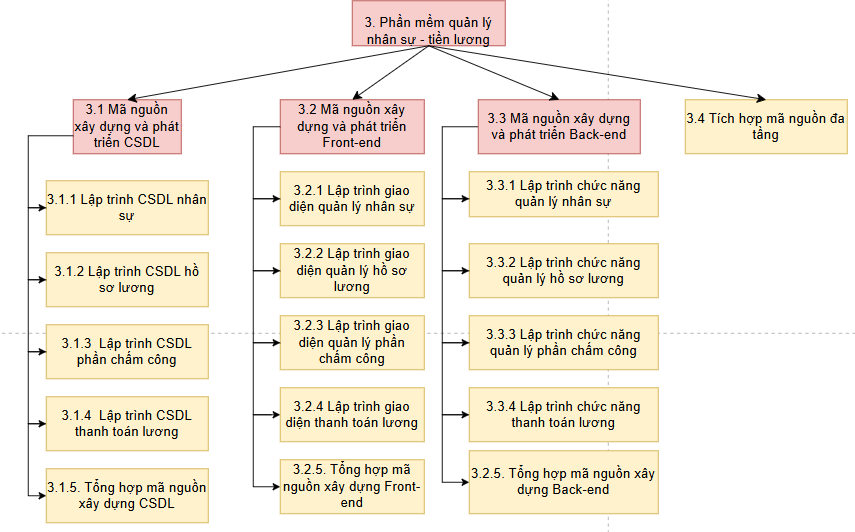
\includegraphics[width=\textwidth]{images/pmquanlyns-tl.png}
    \caption{Phân rã chi tiết phần mềm quản lý nhân sự - tiền lương}
\end{figure}
\begin{figure}[H]
    \centering
    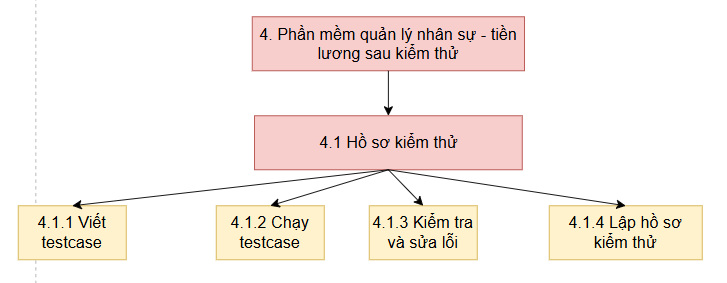
\includegraphics[width=\textwidth]{images/pmsaukiemthu.png}
    \caption{Phân rã chi tiết phần mềm quản lý nhân sự - tiền lương sau kiểm thử}
\end{figure}
\begin{figure}[H]
    \centering
    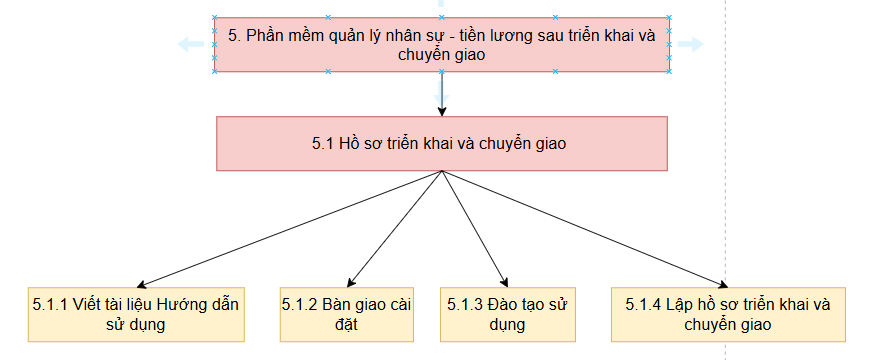
\includegraphics[width=\textwidth]{images/pmsautrienkhai.png}
    \caption{Phân rã chi tiết phần mềm quản lý nhân sự - tiền lương sau triển khai và chuyển giao}
\end{figure}
\subsection{Biên bản phạm vi công việc}
\subsubsection{Xác định mục tiêu và đối tượng khảo sát}
% Viết biên bản phạm vi công việc
\section{Kế hoạch quản lý thời gian}
\subsection{Bảng phụ thuộc công việc và quan hệ thời gian}
% Viết bảng phụ thuộc
\subsection{Sơ đồ AOA và AON}
\subsubsection{Sơ đồ AOA}
\begin{figure}[H]
    \centering
    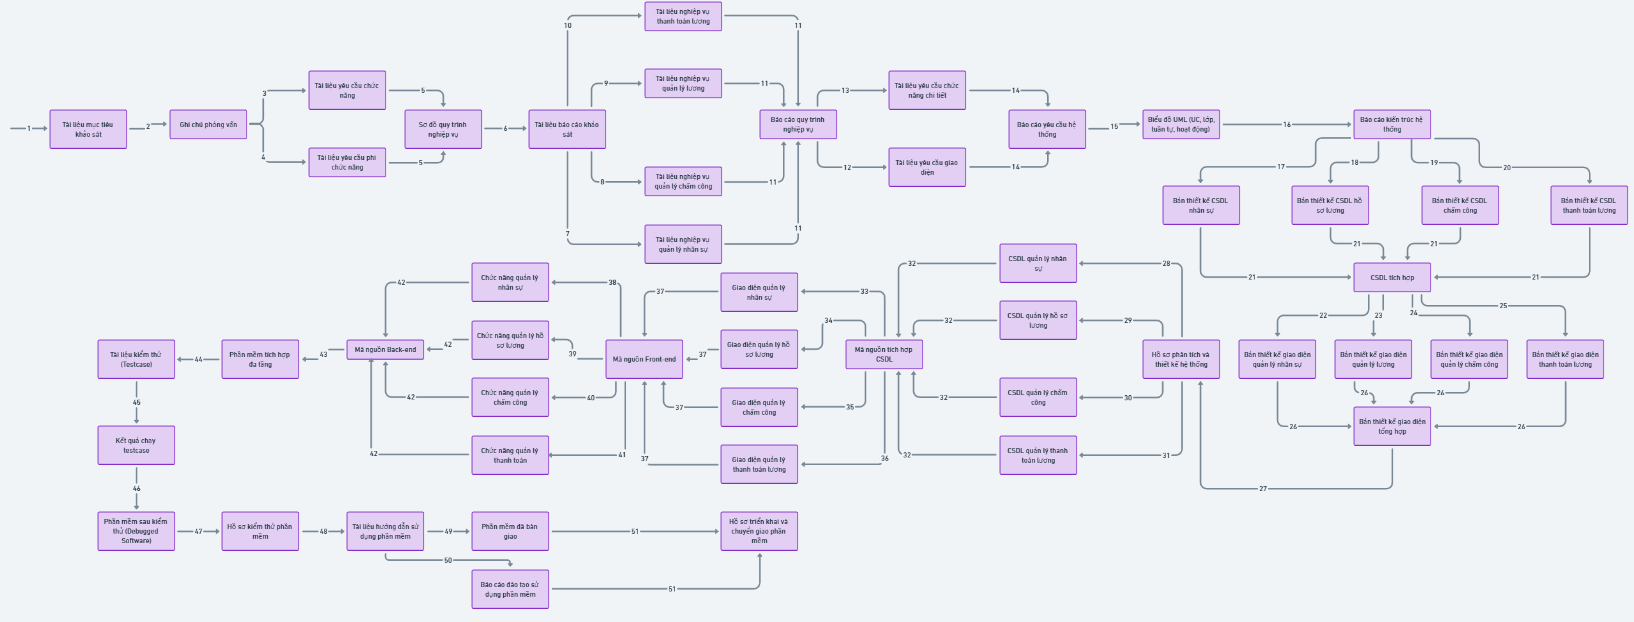
\includegraphics[width=\textwidth]{images/aoa.png}
    \caption{Sơ đồ AOA}
\end{figure}
\subsubsection{Sơ đồ AON}
\begin{figure}[H]
    \centering
    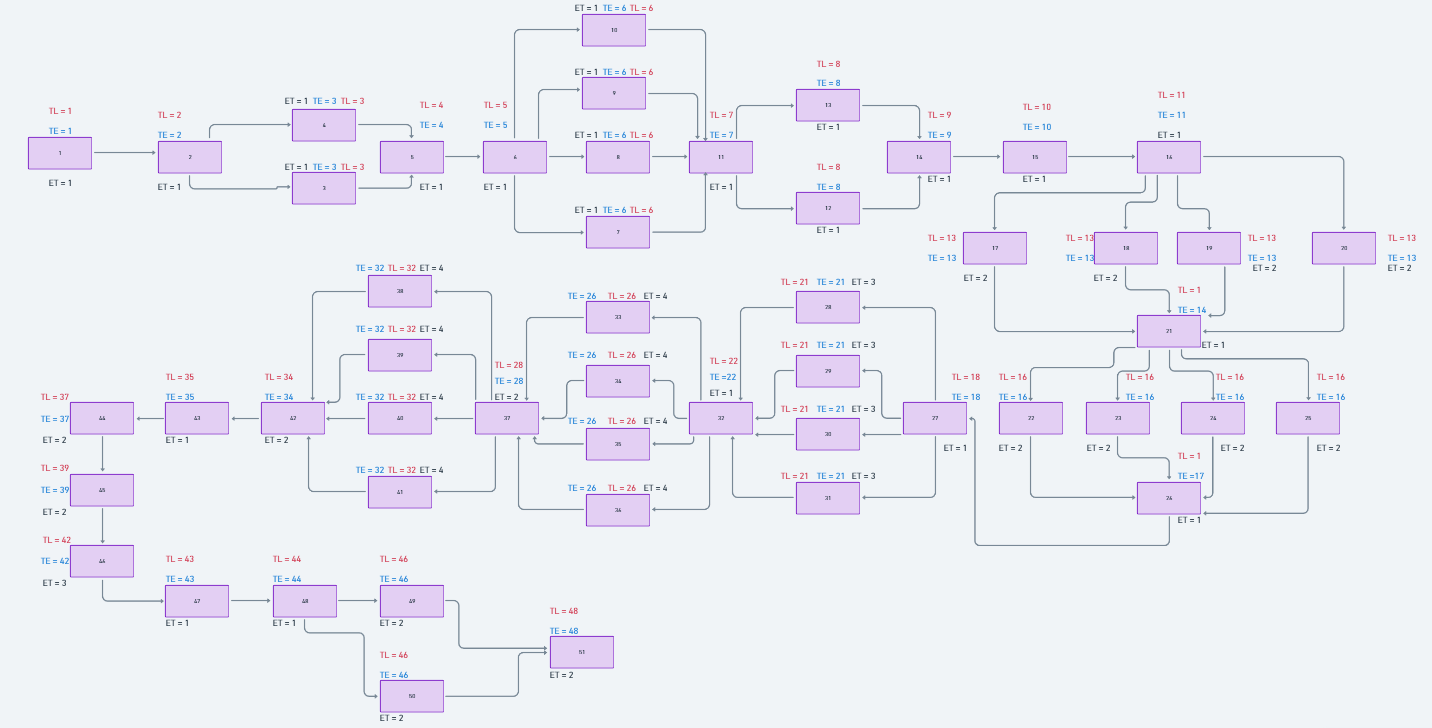
\includegraphics[width=\textwidth]{images/aon.png}
    \caption{Sơ đồ AON}
\end{figure}
\subsection{Sơ đồ Gantt}
\begin{figure}[H]
    \centering
    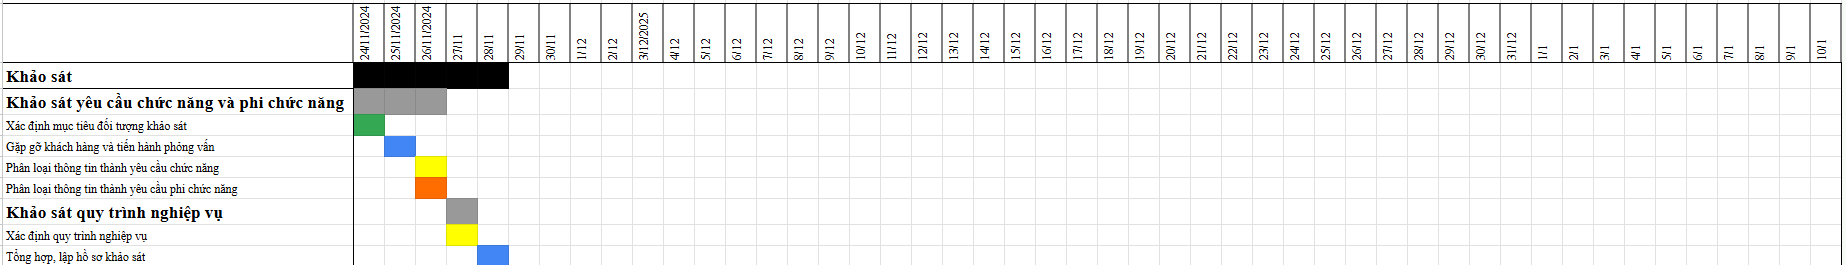
\includegraphics[width=\textwidth]{images/gantt1.png}
    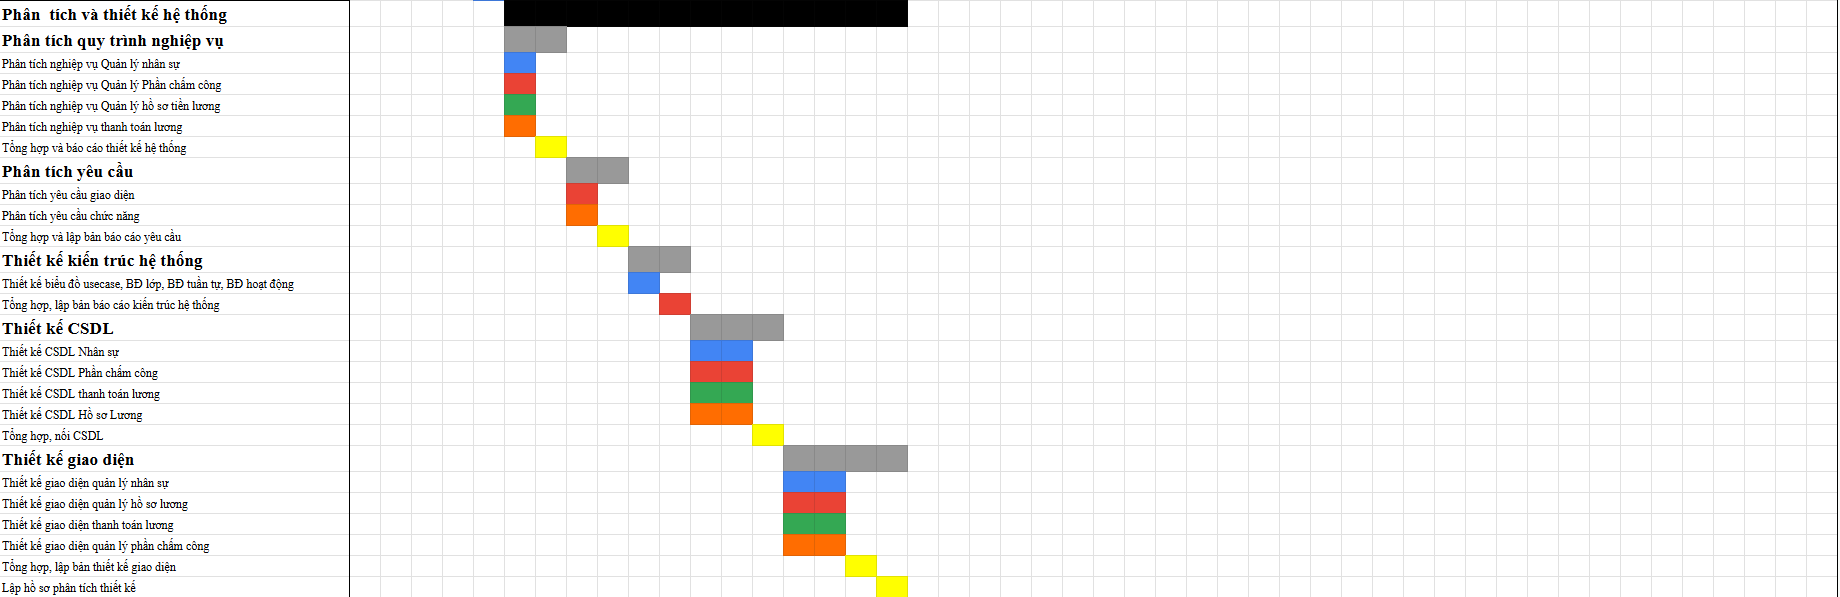
\includegraphics[width=\textwidth]{images/gantt2.png}
    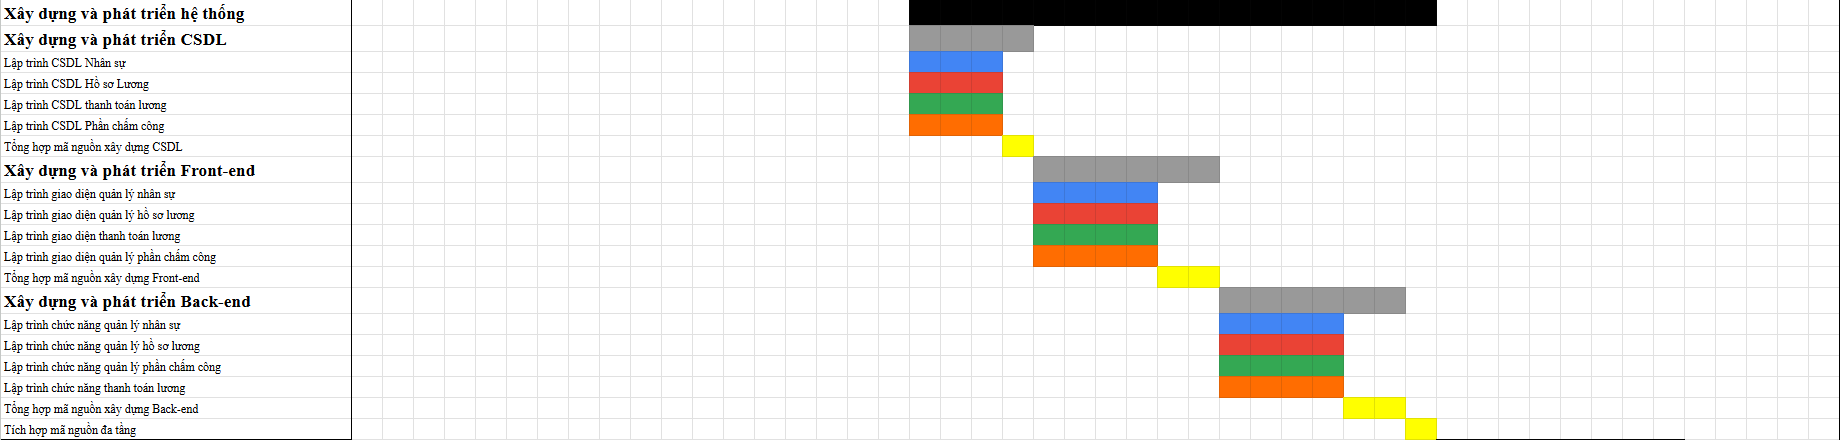
\includegraphics[width=\textwidth]{images/gantt3.png}
    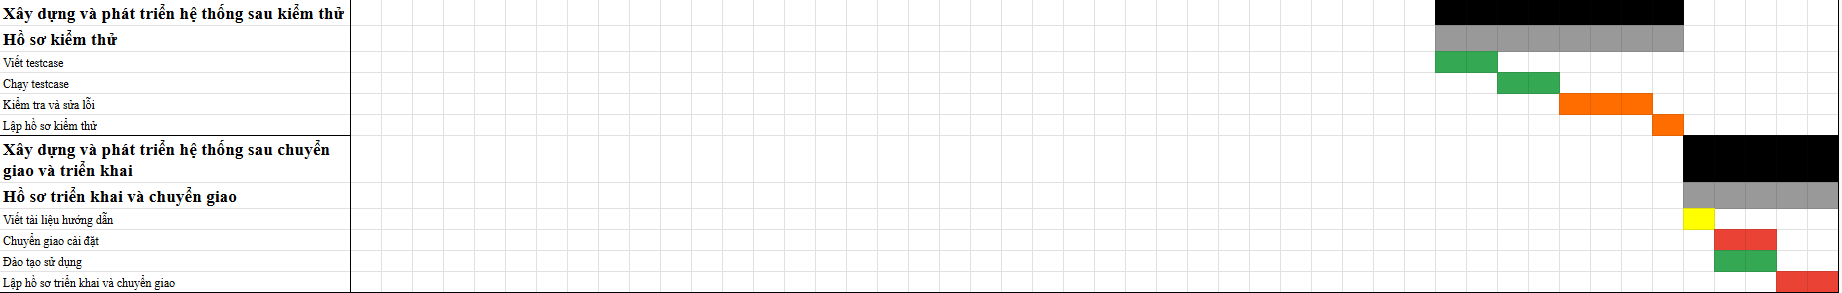
\includegraphics[width=\textwidth]{images/gantt4.png}
    \caption{Sơ đồ Gantt}
\end{figure}
\begin{figure}[H]
    \centering
    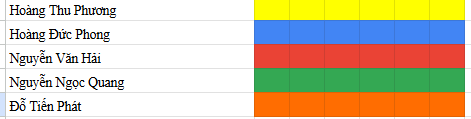
\includegraphics[width=\textwidth]{images/gantt_tv.png}
\end{figure}
\subsection{Tổng kết kế hoạch quản lý thời gian}
% Viết bảng kế hoạch
\section{Kế hoạch quản lý chi phí}
\subsection{Kế hoạch cho nguồn tài nguyên}
\subsubsection{Tài sản cố định}
\begin{itemize}
    \item Các thiết bị phần cứng: máy chấm công.
\end{itemize}

\subsubsection{Chi phí vận hành}
\begin{itemize}
    \item Trả lương quản lý.
    \item Trả lương công việc.
\end{itemize}

\subsubsection{Chi phí phần mềm}
\begin{itemize}
    \item Domain, Hosting, Server
\end{itemize}

\subsubsection{Phúc lợi và hoạt động khác}
\begin{itemize}
    \item Liên hoan cuối tháng.
    \item Lương thưởng.
\end{itemize}

\subsection{Ước lượng chi phí}
\begin{table}[H]
    \caption{Ước lượng chi phí}
    \centering
    \renewcommand{\arraystretch}{1.5} % Tăng khoảng cách giữa các dòng
    \begin{tabular}{|c|c|}
        \hline
        \textbf{Đầu mục chi phí}                  & \textbf{Chi phí ước tính (VNĐ)} \\
        \hline
        Tài sản cố định                           & 44.400.000                      \\
        \hline
        Chi phí vận hành                          & 113.600.000                     \\
        \hline
        Chi phí phần mềm                          & 40.000.000                      \\
        \hline
        Phúc lợi và hoạt động khác                & 62.000.000                      \\
        \hline
        \multicolumn{1}{|c|}{\textbf{Tổng cộng:}} & \textbf{260.000.000}            \\
        \hline
    \end{tabular}
\end{table}

\subsection{Dự toán chi phí}
\subsubsection{Tài sản cố định}
\begin{table}[H]
    \caption{Dự toán chi phí tài sản cố định}
    \centering
    \renewcommand{\arraystretch}{1.5} % Tăng khoảng cách giữa các hàng
    \begin{tabular}{|c|c|c|c|c|}
        \hline
        \textbf{Hạng mục}                        & \textbf{Số lượng}   & \textbf{Đơn giá (VNĐ)} & \textbf{Đơn vị tính} & \textbf{Thành tiền (VNĐ)} \\
        \hline
        Máy chấm công                            & 1                   & 44.400.000             & Thiết bị             & 44.400.000                \\
        \hline
        \multicolumn{4}{|c|}{\textbf{Tổng cộng}} & \textbf{44.400.000}                                                                             \\
        \hline
    \end{tabular}
\end{table}


\subsubsection{Chi phí vận hành}
A. Trả lương quản lý
\begin{table}[H]
    \centering
    \renewcommand{\arraystretch}{1.5} % Tăng khoảng cách giữa các hàng
    \begin{tabular}{|p{3cm}|p{2.5cm}|p{2.3cm}|p{2cm}|p{3cm}|}
        \hline
        \textbf{Họ tên}                           & \textbf{Vị trí}     & \textbf{Mức lương (VND/Ngày)} & \textbf{Thời gian quản lý dự án (ngày)} & \textbf{Chi phí quản lý thực tế (VNĐ)} \\
        \hline
        Hoàng Thu Phương                          & Quản lý dự án       & 1.000.000                     & 48                                      & 48.000.000                             \\
        \hline
        \multicolumn{4}{|c|}{\textbf{Tổng cộng:}} & \textbf{48.000.000}                                                                                                                    \\
        \hline
    \end{tabular}
    \caption{Chi phí trả lương quản lý}
\end{table}

B. Trả lương công việc
\begin{table}[H]
    \centering
    \renewcommand{\arraystretch}{1.5} % Tăng khoảng cách giữa các hàng
    \caption{Bảng lương cơ bản theo vị trí}
    \begin{tabular}{|c|c|c|}
        \hline
        \textbf{Vị trí} & \textbf{Mức lương (VNĐ/Ngày)} & \textbf{Lương (VNĐ/Tháng)} \\
        \hline
        Quản lý dự án   & 1.000.000                     & 30.000.000                 \\
        \hline
        Nhân viên       & 600.000                       & 18.000.000                 \\
        \hline
    \end{tabular}
\end{table}

\clearpage
\begin{longtable}{|c|p{3cm}|c|c|c|c|p{3cm}|}
    \caption{WBS - Chi phí thực tế theo công việc}                                                                                                                                                                                                                                                         \\
    \hline
    \multirow{2}{*}{\textbf{WBS}}   & \multirow{2}{*}{\textbf{Tên công việc}}                       & \multicolumn{2}{c|}{\textbf{Thời gian (ngày)}} & \multicolumn{2}{c|}{\textbf{Số người tham gia}} & \multirow{2}{*}{\parbox{3cm}{\centering \textbf{Chi phí thực tế                                   \\ (VNĐ)}}} \\ \cline{3-6}
                                    &                                                               & \textbf{Kế hoạch}                              & \textbf{Thực tế}                                & \textbf{Quản lý}                                                & \textbf{Nhân viên} &            \\ \hline
    \endfirsthead
    \hline
    \multirow{2}{*}{\textbf{WBS}}   & \multirow{2}{*}{\textbf{Tên công việc}}                       & \multicolumn{2}{c|}{\textbf{Thời gian (ngày)}} & \multicolumn{2}{c|}{\textbf{Số người tham gia}} & \multirow{2}{*}{\parbox{3cm}{\centering \textbf{Chi phí thực tế                                   \\ (VNĐ)}}} \\ \cline{3-6}
                                    &                                                               & \textbf{Kế hoạch}                              & \textbf{Thực tế}                                & \textbf{Quản lý}                                                & \textbf{Nhân viên} &            \\ \hline
    \endhead
    \hline \multicolumn{7}{|r|}{{Tiếp theo trang sau}}                                                                                                                                                                                                                                                     \\ \hline
    \endfoot
    \hline
    \endlastfoot
    1                               & Khảo sát                                                      & 5                                              & 5                                               & 1                                                               & 3                  & 4.400.000  \\ \hline
    1.1                             & Khảo sát yêu cầu chức năng và phi chức năng                   & 3                                              & 3                                               & 1                                                               & 3                  & 2.800.000  \\ \hline
    1.1.1                           & Xác định mục tiêu và đối tượng khảo sát                       & 1                                              & 1                                               & 0                                                               & 1                  & 600.000    \\ \hline
    1.1.2                           & Gặp gỡ khách hàng và tiến hành phỏng vấn                      & 1                                              & 1                                               & 0                                                               & 1                  & 600.000    \\ \hline
    1.1.3                           & Phân loại thông tin thành yêu cầu chức năng                   & 1                                              & 1                                               & 1                                                               & 0                  & 1.000.000  \\ \hline
    1.1.4                           & Phân loại thông tin thành yêu cầu phi chức năng               & 1                                              & 1                                               & 0                                                               & 1                  & 600.000    \\ \hline
    1.2                             & Khảo sát quy trình nghiệp vụ                                  & 1                                              & 1                                               & 1                                                               & 0                  & 1.000.000  \\ \hline
    1.2.1                           & Xác định quy trình nghiệp vụ                                  & 1                                              & 1                                               & 1                                                               & 0                  & 1.000.000  \\ \hline
    1.3                             & Tổng hợp, lập hồ sơ khảo sát                                  & 1                                              & 1                                               & 0                                                               & 1                  & 600.000    \\ \hline
    2                               & Phân tích và Thiết kế hệ thống                                & 13                                             & 13                                              & 1                                                               & 4                  & 19.400.000 \\ \hline
    2.1                             & Phân tích quy trình nghiệp vụ                                 & 2                                              & 2                                               & 1                                                               & 4                  & 3.400.000  \\ \hline
    2.1.1                           & Phân tích nghiệp vụ Quản lý nhân sự                           & 1                                              & 1                                               & 0                                                               & 1                  & 600.000    \\ \hline
    2.1.2                           & Phân tích nghiệp vụ Quản lý Phần chấm công                    & 1                                              & 1                                               & 0                                                               & 1                  & 600.000    \\ \hline
    2.1.3                           & Phân tích nghiệp vụ Quản lý hồ sơ tiền lương                  & 1                                              & 1                                               & 0                                                               & 1                  & 600.000    \\ \hline
    2.1.4                           & Phân tích nghiệp vụ thanh toán lương                          & 1                                              & 1                                               & 0                                                               & 1                  & 600.000    \\ \hline
    2.1.5                           & Tổng hợp và báo cáo thiết kế hệ thống                         & 1                                              & 1                                               & 1                                                               & 0                  & 1.000.000  \\ \hline
    2.2                             & Phân tích yêu cầu                                             & 2                                              & 2                                               & 1                                                               & 2                  & 2.200.000  \\ \hline
    2.2.1                           & Phân tích yêu cầu giao diện                                   & 1                                              & 1                                               & 0                                                               & 1                  & 600.000    \\ \hline
    2.2.2                           & Phân tích yêu cầu chức năng                                   & 1                                              & 1                                               & 0                                                               & 1                  & 600.000    \\ \hline
    2.2.3                           & Tổng hợp và lập bản báo cáo yêu cầu                           & 1                                              & 1                                               & 1                                                               & 0                  & 1.000.000  \\ \hline
    2.3                             & Thiết kế kiến trúc hệ thống                                   & 2                                              & 2                                               & 0                                                               & 2                  & 1.200.000  \\ \hline
    2.3.1                           & Thiết kế biểu đồ usecase, BĐ lớp, BĐ tuần tự, BĐ hoạt động    & 1                                              & 1                                               & 0                                                               & 1                  & 600.000    \\ \hline
    2.3.2                           & Tổng hợp, lập bản báo cáo kiến trúc hệ thống                  & 1                                              & 1                                               & 0                                                               & 1                  & 600.000    \\ \hline
    2.4                             & Thiết kế CSDL                                                 & 3                                              & 3                                               & 1                                                               & 4                  & 5.800.000  \\ \hline
    2.4.1                           & Thiết kế CSDL Nhân sự                                         & 2                                              & 2                                               & 0                                                               & 1                  & 1.200.000  \\ \hline
    2.4.2                           & Thiết kế CSDL Hồ sơ Lương                                     & 2                                              & 2                                               & 0                                                               & 1                  & 1.200.000  \\ \hline
    2.4.3                           & Thiết kế CSDL Phần chấm công                                  & 2                                              & 2                                               & 0                                                               & 1                  & 1.200.000  \\ \hline
    2.4.4                           & Thiết kế CSDL thanh toán lương                                & 2                                              & 2                                               & 0                                                               & 1                  & 1.200.000  \\ \hline
    2.4.5                           & Tổng hợp, nối CSDL                                            & 1                                              & 1                                               & 1                                                               & 0                  & 1.000.000  \\ \hline
    2.5                             & Thiết kế giao diện                                            & 4                                              & 4                                               & 1                                                               & 4                  & 5.800.000  \\ \hline
    2.5.1                           & Thiết kế giao diện quản lý nhân sự                            & 2                                              & 2                                               & 0                                                               & 1                  & 1.200.000  \\ \hline
    2.5.2                           & Thiết kế giao diện quản lý hồ sơ lương                        & 2                                              & 2                                               & 0                                                               & 1                  & 1.200.000  \\ \hline
    2.5.3                           & Thiết kế giao diện quản lý phần chấm công                     & 2                                              & 2                                               & 0                                                               & 1                  & 1.200.000  \\ \hline
    2.5.4                           & Thiết kế giao diện thanh toán lương                           & 2                                              & 2                                               & 0                                                               & 1                  & 1.200.000  \\ \hline
    2.5.5                           & Tổng hợp, lập bản thiết kế giao diện                          & 1                                              & 1                                               & 1                                                               & 0                  & 1.000.000  \\ \hline
    2.6                             & Lập hồ sơ phân tích thiết kế                                  & 1                                              & 1                                               & 1                                                               & 0                  & 1.000.000  \\ \hline
    3                               & Xây dựng và phát triển hệ thống                               & 17                                             & 17                                              & 1                                                               & 4                  & 32.400.000 \\ \hline
    3.1                             & Xây dựng và phát triển CSDL                                   & 4                                              & 4                                               & 1                                                               & 4                  & 8.200.000  \\ \hline
    3.1.1                           & Lập trình CSDL Nhân sự                                        & 3                                              & 3                                               & 0                                                               & 1                  & 1.800.000  \\ \hline
    3.1.2                           & Lập trình CSDL Hồ sơ Lương                                    & 3                                              & 3                                               & 0                                                               & 1                  & 1.800.000  \\ \hline
    3.1.3                           & Lập trình CSDL Phần chấm công                                 & 3                                              & 3                                               & 0                                                               & 1                  & 1.800.000  \\ \hline
    3.1.4                           & Lập trình CSDL thanh toán lương                               & 3                                              & 3                                               & 0                                                               & 1                  & 1.800.000  \\ \hline
    3.1.5                           & Tổng hợp mã nguồn xây dựng CSDL                               & 1                                              & 1                                               & 1                                                               & 0                  & 1.000.000  \\ \hline
    3.2                             & Xây dựng và phát triển Front-end                              & 6                                              & 6                                               & 1                                                               & 4                  & 11.600.000 \\ \hline
    3.2.1                           & Lập trình giao diện quản lý nhân sự                           & 4                                              & 4                                               & 0                                                               & 1                  & 2.400.000  \\ \hline
    3.2.2                           & Lập trình giao diện quản lý hồ sơ lương                       & 4                                              & 4                                               & 0                                                               & 1                  & 2.400.000  \\ \hline
    3.2.3                           & Lập trình giao diện quản lý phần chấm công                    & 4                                              & 4                                               & 0                                                               & 1                  & 2.400.000  \\ \hline
    3.2.4                           & Lập trình giao diện thanh toán lương                          & 4                                              & 4                                               & 0                                                               & 1                  & 2.400.000  \\ \hline
    3.2.5                           & Tổng hợp mã nguồn xây dựng Front-end                          & 2                                              & 2                                               & 1                                                               & 0                  & 2.000.000  \\ \hline
    3.3                             & Xây dựng và phát triển Back-end                               & 7                                              & 7                                               & 1                                                               & 4                  & 11.600.000 \\ \hline
    3.3.1                           & Lập trình chức năng quản lý nhân sự                           & 4                                              & 4                                               & 0                                                               & 1                  & 2.400.000  \\ \hline
    3.3.2                           & Lập trình chức năng quản lý hồ sơ lương                       & 4                                              & 4                                               & 0                                                               & 1                  & 2.400.000  \\ \hline
    3.3.3                           & Lập trình chức năng quản lý phần chấm công                    & 4                                              & 4                                               & 0                                                               & 1                  & 2.400.000  \\ \hline
    3.3.4                           & Lập trình chức năng thanh toán lương                          & 4                                              & 4                                               & 0                                                               & 1                  & 2.400.000  \\ \hline
    3.3.5                           & Tổng hợp mã nguồn xây dựng Back-end                           & 2                                              & 2                                               & 1                                                               & 0                  & 2.000.000  \\ \hline
    3.4                             & Tích hợp mã nguồn đa tầng                                     & 1                                              & 1                                               & 1                                                               & 0                  & 1.000.000  \\ \hline
    4                               & Xây dựng và phát triển phần mềm sau kiểm thử                  & 8                                              & 8                                               & 0                                                               & 2                  & 4.800.000  \\ \hline
    4.1                             & Hồ sơ kiểm thử                                                & 8                                              & 8                                               & 0                                                               & 2                  & 4.800.000  \\ \hline
    4.1.1                           & Viết testcase                                                 & 2                                              & 2                                               & 0                                                               & 1                  & 1.200.000  \\ \hline
    4.1.2                           & Chạy testcase                                                 & 2                                              & 2                                               & 0                                                               & 1                  & 1.200.000  \\ \hline
    4.1.3                           & Kiểm tra và sửa lỗi                                           & 3                                              & 3                                               & 0                                                               & 1                  & 1.800.000  \\ \hline
    4.1.4                           & Lập hồ sơ kiểm thử                                            & 1                                              & 1                                               & 0                                                               & 1                  & 600.000    \\ \hline
    5                               & Xây dựng và phát triển phần mềm sau triển khai và chuyển giao & 5                                              & 5                                               & 1                                                               & 2                  & 4.600.000  \\ \hline
    5.1                             & Hồ sơ triển khai và chuyển giao                               & 5                                              & 5                                               & 1                                                               & 2                  & 4.600.000  \\ \hline
    5.1.1                           & Viết tài liệu hướng dẫn                                       & 1                                              & 1                                               & 1                                                               & 0                  & 1.000.000  \\ \hline
    5.1.2                           & Chuyển giao cài đặt                                           & 2                                              & 2                                               & 0                                                               & 1                  & 1.200.000  \\ \hline
    5.1.3                           & Đào tạo sử dụng                                               & 2                                              & 2                                               & 0                                                               & 1                  & 1.200.000  \\ \hline
    5.1.4                           & Lập hồ sơ triển khai và chuyển giao                           & 2                                              & 2                                               & 0                                                               & 1                  & 1.200.000  \\ \hline
    \multicolumn{6}{|c|}{Tổng cộng} & 65.600.000                                                                                                                                                                                                                                                           \\ \hline
\end{longtable}

\begin{tabbing}
    Tổng CPVH (*): 65.600.000 + 48.000.000 = \= 113.600.000 (VNĐ) \\
    *: Chi phí vận hành gồm: Chi phí quản lý và chi phí thực tế theo phân chia công việc \\
    ( được trình bày ở phần B.Trả lương công việc ) %  % Dòng này sẽ xuống dòng nhưng vẫn thẳng hàng
\end{tabbing}

\subsubsection{Chi phí phần mềm}
\begin{table}[H]
    \centering
    \renewcommand{\arraystretch}{1.5} % Tăng khoảng cách giữa các hàng
    \caption{Dự toán chi phí phần mềm}
    \begin{tabular}{|c|c|c|c|c|}
        \hline
        \textbf{Hạng mục}                         & \textbf{Số lượng}   & \textbf{Đơn giá (VNĐ)} & \textbf{Đơn vị tính} & \textbf{Thành tiền (VNĐ)} \\
        \hline
        Domain                                    & 1                   & 500.000                & Năm                  & 500.000                   \\
        \hline
        Hosting                                   & 1                   & 1.500.000              & Năm                  & 1.500.000                 \\
        \hline
        Server                                    & 1                   & 38.000.000             & Năm                  & 38.000.000                \\
        \hline
        \multicolumn{4}{|c|}{\textbf{Tổng cộng:}} & \textbf{40.000.000}                                                                             \\
        \hline
    \end{tabular}
\end{table}


\subsubsection{Phúc lợi và hoạt động khác}
\begin{table}[H]
    \centering
    \renewcommand{\arraystretch}{1.5} % Tăng khoảng cách giữa các hàng
    \caption{Dự toán chi phí phúc lợi và hoạt động khác}
    \begin{tabular}{|c|c|c|c|c|}
        \hline
        \textbf{Hạng mục}                         & \textbf{Số lượng}   & \textbf{Đơn giá (VNĐ)} & \textbf{Đơn vị tính} & \textbf{Thành tiền (VNĐ)} \\
        \hline
        Liên hoan cuối tháng                      & 2                   & 6.000.000              & Tháng                & 12.000.000                \\
        \hline
        Lương thưởng                              & 1                   & 50.000.000             & Lần                  & 50.000.000                \\
        \hline
        \multicolumn{4}{|c|}{\textbf{Tổng cộng:}} & \textbf{62.000.000}                                                                             \\
        \hline
    \end{tabular}
\end{table}

\subsection{Quản lý chi phí chia theo giai đoạn dự án}
\subsubsection{Bảng phân bổ chi phí theo giai đoạn dự án}
\begin{table}[H]
    \centering
    \renewcommand{\arraystretch}{1.5} % Tăng khoảng cách giữa các hàng
    \caption{Bảng phân bổ chi phí theo giai đoạn dự án}
    \begin{tabular}{|c|c|}
        \hline
        \textbf{Giai đoạn}                        & \textbf{Chi phí (VNĐ)} \\
        \hline
        Khảo sát                                  & 9.400.000              \\
        \hline
        Phân tích và Thiết kế                     & 76.800.000             \\
        \hline
        Xây dựng và phát triển                    & 89.400.000             \\
        \hline
        Kiểm thử                                  & 18.800.000             \\
        \hline
        Triển khai và bàn giao                    & 65.600.000             \\
        \hline
        \multicolumn{1}{|c|}{\textbf{Tổng cộng:}} & \textbf{260.000.000}   \\
        \hline
    \end{tabular}
\end{table}


\subsubsection{Quản lý chi phí chi tiết theo giai đoạn dự án}
Giai đoạn 1: Khảo sát
\begin{tabbing}
    Thời gian: \= 5 ngày. \\
    Chi phí chi tiết: %  % Dòng này sẽ xuống dòng nhưng vẫn thẳng hàng
\end{tabbing}
\begin{itemize}
    \item Chi phí nhân sự: 4.400.000 VNĐ.
    \item Chi phí quản lý: 5.000.000 VNĐ.
    \item Tổng chi phí: 9.400.000 VNĐ.
\end{itemize}

Giai đoạn 2: Phân tích và Thiết kế
\begin{tabbing}
    Thời gian: \= 13 ngày. \\
    Chi phí chi tiết: %  % Dòng này sẽ xuống dòng nhưng vẫn thẳng hàng
\end{tabbing}
\begin{itemize}
    \item Chi phí nhân sự: 19.400.000 VNĐ.
    \item Chi phí quản lý: 13.000.000 VNĐ.
    \item Chi phí mua thiết bị phần cứng (Máy chấm công): 44.400.000 VNĐ.
    \item Tổng chi phí: 76.800.000 VNĐ.
\end{itemize}

Giai đoạn 3: Xây dựng và phát triển
\begin{tabbing}
    Thời gian: \= 17 ngày. \\
    Chi phí chi tiết: %  % Dòng này sẽ xuống dòng nhưng vẫn thẳng hàng
\end{tabbing}
\begin{itemize}
    \item Chi phí nhân sự: 32.400.000 VNĐ.
    \item Chi phí quản lý: 17.000.000 VNĐ.
    \item Chi phí phần mềm (Hosting, Server, Domain): 40.000.000 VNĐ.
    \item Tổng chi phí: 89.400.000 VNĐ.
\end{itemize}

Giai đoạn 4: Kiểm thử
\begin{tabbing}
    Thời gian: \= 8 ngày. \\
    Chi phí chi tiết: %  % Dòng này sẽ xuống dòng nhưng vẫn thẳng hàng
\end{tabbing}
\begin{itemize}
    \item Chi phí nhân sự: 4.800.000 VNĐ.
    \item Chi phí quản lý: 8.000.000 VNĐ.
    \item Chi phí liên hoan: 6.000.000 VNĐ.
    \item Tổng chi phí: 18.800.000 VNĐ.
\end{itemize}

Giai đoạn 5: Triển khai và bàn giao
\begin{tabbing}
    Thời gian: \= 5 ngày. \\
    Chi phí chi tiết: %  % Dòng này sẽ xuống dòng nhưng vẫn thẳng hàng
\end{tabbing}
\begin{itemize}
    \item Chi phí nhân sự: 4.600.000 VNĐ.
    \item Chi phí quản lý: 5.000.000 VNĐ.
    \item Chi phí phúc lợi và hoạt động khác (Liên hoan, lương thưởng): 56.000.000 VNĐ.
    \item Tổng chi phí: 65.600.000 VNĐ.
\end{itemize}

\subsubsection{Tổng chi phí dự án}
\begin{itemize}
    \item Tổng chi phí nhân sự: 65.600.000 VNĐ
    \item Tổng chi phí quản lý: 48.000.000 VNĐ
    \item Tổng chi phí mua thiết bị: 44.400.000 VNĐ
    \item Tổng chi phí phần mềm: 40.000.000 VNĐ
    \item Tổng chi phí phúc lợi và hoạt động khác: 62.000.000 VNĐ
\end{itemize}
\textbf{Tổng chi phí dự án: 260.000.000 VNĐ}
